%% This document gives an example on how to use the ntnubachelorthesis
%% LaTeX document class.
%% Use oneside for PDF delivery and twoside for printing in a book style
%% use language english, norsk, nynorsk and one of the following shortenings
%%  ``BSP'' Bachelor i Spillprogrammering,\\
%%  ``BRD'' Bachelor i drift av nettverk og datasystemer,\\
%%  ``BIS'' Bachelor i Informasjonssikkerhet,\\
%%  ``BPU'' Bachelor i Programvareutvikling, \\
%%  ``BIND'' Bachelor i Ingeniorfad - data, \\
%%  ``BADR'' Bachelor i drift av datasystemer, \\
%%  ``BIT'' Bachelor i informatikk, \\
%%  ``BABED'' Bachelor i IT-støttet bedriftsutvikling.
%%   for example \documentclass[BIS,norsk,twoside]{ntnuthesis/ntnubachelorthesis}

\documentclass[BIS,norsk,oneside]{ntnuthesis/ntnubachelorthesis}
\thesistitle{Case 3: Misbruk av NTNU sin infrastruktur til utvinning av kryptovaluta}
\thesisshorttitle{Case 3: Misbruk av NTNU sin infrastruktur til utvinning av kryptovaluta}
\thesisauthor{Philip Nyblom, Fredrik Theien, Thomas Huse, Ole Martin Søgnen}
\thesisdate{16.05.2018}

\usepackage{csvsimple}
\usepackage{booktabs}
\usepackage{gnuplottex}
\usepackage[T1]{fontenc}
\usepackage[utf8]{inputenc}     % For utf8 encoded .tex files because...
\usepackage[norsk]{babel}       % For Norwegian labeling
\usepackage{graphicx}           % For inclusion of graphics
\PassOptionsToPackage{hyphens}{url}
\usepackage{url}
\usepackage{hyperref}    % For cross references in pdf
\usepackage{tabularx}
\usepackage[table]{xcolor}
\usepackage{colortbl}
\usepackage{placeins}
\usepackage{pdfpages}
\usepackage{enumitem}
\usepackage{multirow}
\usepackage{lscape}
\usepackage{bigstrut}
\usepackage{verbatim}
\usepackage{float}


\definecolor{darkgreen}{rgb}{0,0.5,0}
\definecolor{darkred}{rgb}{0.5,0.0,0}

\lstset{        basicstyle=\ttfamily,
                keywordstyle=\color{blue}\ttfamily,
                stringstyle=\color{darkred}\ttfamily,
                commentstyle=\color{darkgreen}\ttfamily,
}


%Typesetting of C++
\newcommand{\CPP}[0]{{C\nolinebreak[4]\hspace{-.1em}\raisebox{.1ex}{\small\bf +\hspace{-.1em}+\ }}}



%\newcommand{\comment}[1]{\textcolor{blue}{\emph{#1}}}  %% use of the colour and you can see how to use commands with parts \comment{so what}

%% The class files defines these two
%% \newcommand{\NTNU}{Norwegian University for Science and Technology} %

% you can create you one #define like structures using the \newcommand feature
% you can change behaviour using \renewcommand

\newcommand{\com}[1]{{\color{red}#1}} % supervisor comment
%\renewcommand{\com}[1]{} %remove starting % to remove supervisor comments
% This will appear in text \com{Lecuters comment} and be visible unless you uncomment
% the renewcommand line.

\newcommand{\todo}[1]{{\color{green}#1}} % items to do
%\renewcommand{\todo}[1]{} %remove starting % to remove items to do

\newcommand{\n}[1]{{\color{blue}#1}} % other comment
%\renewcommand{\n}[1]{} %remove starting % to remove notes

\newcommand{\dn}[1]{} % add the d to a note to say that you have finished with it.

\newcommand{\gj}{NTNU i Gj\o{}vik}


% Norwegian Characters,  needs the {} or to be separate from the next letters
% \o{}   \aa{}   \ae{}   so at the end of a word you can use \o  \aa   \ae
% \O{}   \AA{}   \AE{}   you can also just leave a space and latex will remove it
%    eg, NTNU i Gj\o vik  or NTNU i Gj\o{}vik

\graphicspath{ {bilder/} }

\begin{document}

\thesistitlepage

\tableofcontents
\listoffigures
\listoftables

%\chapter*{Kortfattet sammendrag}
Kommer...
\chapter{Introduksjon}
%--------------------MÅ INN I HOVEDRAPPORT------------------------------------------
Rotårsaksanalyser er et lite brukt verktøy innen informasjonssikkerhet, men er av økende betydning. Vanlig tilnærming til informasjonssikkerhetsstyring er å utføre en risiko- og sårbarhetsanalyse (ROS-analyse) for så å gjennomføre tiltak som fører risikoene til et akseptabelt nivå. En annen hyppig brukt tilnærming er hendelseshåndtering der en planlegger hvordan det skal responderes på hendelser etter de er inntruffet. Rotårsaksanalyse skiller seg fra disse ved å gå i dybden på problemet, kartlegge hva slags rotårsaker som står bak, og innføre tiltak for å fjerne disse helt.
%%%%%%%%%%%%%%%%%%%%%%%%%%%%%%%%%%%%%%%%%%%%%%%%%%%%%%%%%%%%%%%%%%%%%%%%%%%%%%%%%%%%%

\section{Oppgavebeskrivelse}
Denne rapporten er en delrapport i en større oppgave om rotårsaksanalyse. Dette caset går inn på rotårsaken til misbruk av NTNU sine ressurser og infrastruktur til å grave kryptovaluta. De to siste årene har både verdien og antallet av kryptovaluta økt drastisk. Det finnes per dags dato over 1500 forskjellige kryptovalutaer. Kryptovaluta blir "minet", eller gravet ut, ved bruk av regnekraft. Dette betyr at enhver datamaskin kan delta i utgravingen. Etterhvert vil vanskelighetsgraden for å grave ut nye "coins", eller mynter, øke. Når vanskelighetsgraden øker trenger en mer datakraft og større maskinrigger til å grave ut mynter. 

NTNU forvalter stor regnekraft spredt på flere lokasjoner. NTNU har også hatt supermaskiner før, de har en nå og de får nå en ny supermaskin. Supermaskiner er store datamaskiner på størrelse med et rom, og har enorm datakraft. Disse er spesielt attraktive for aktører å misbruke til å grave etter mynter. Siden trenden har økt de siste årene, og NTNU er i besittelse av mye regnekraft, må NTNU aktivt jobbe for å beskytte infrastrukturen. 

Siden dette er av økende trend, og Seksjon for Digital Sikkerhet har oppdaget at noe av infrastrukturen har blitt brukt til utgraving av kryptovaluta, vil de undersøke måter å eliminere dette misbruket. 

Denne analysen går ut på å identifisere rotårsaken til den økende trenden å bruke NTNU sin infrastruktur til utgraving av kryptovaluta og foreslå tiltak for å eliminere den. I løpet av rapporten ønsker vi å svare på følgende forskningsspørsmål:

\begin{itemize}
    \item 
\end{itemize}

\section{Metode}
Metodebruken i denne analysen er delt inn i syv steg som vist i \hyperref[fig:prosess]{Figur 1} under. I hvert steg av denne prosessen brukes det ulike verktøy for å hjelpe til med å forstå problemet, finne rotårsak, og tilslutt implementere tiltak for å eliminere årsakene. 
\begin{figure}[H]
    \centering
    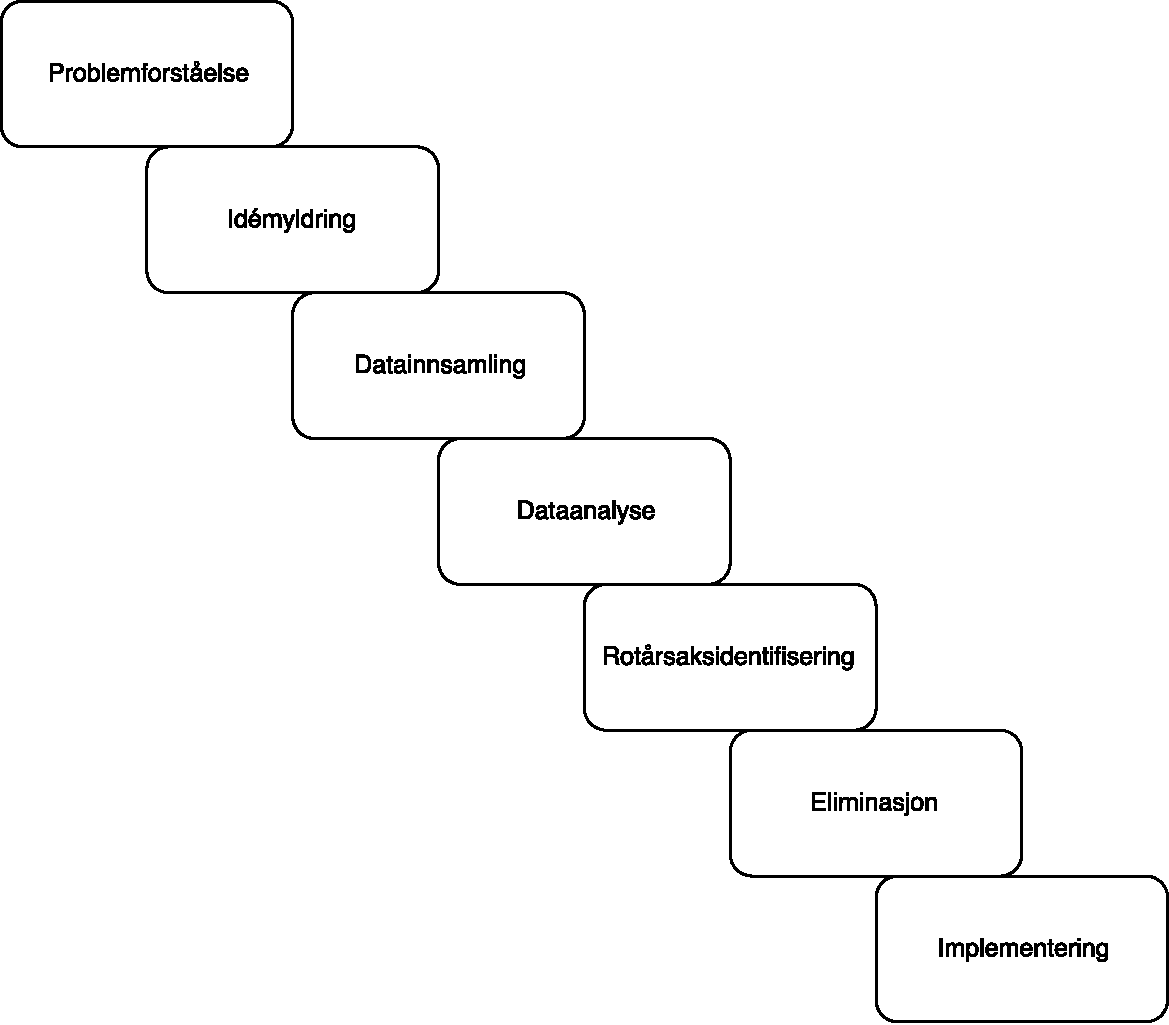
\includegraphics[scale=0.6]{case_1/bilder/prosess.pdf}
    \label{fig:prosess}
    \caption[Rotårsaksanalyseprosessen]{Rotårsaksanalyseprosessen definert av Andersen og Fagerli}
\end{figure}
\chapter{Problemforståelse}

\chapter{Idémyldring}
I dette steget av prosessen er målet å generere en liste over det vi tror kan være mulige årsaker til problemet. Det er en del forskjellige verktøy en kan bruke for å oppnå dette, men vi har valgt å benytte Idémyldring på basis av RCA boken \cite{RCA} sin fremgangsmåte for valg av verktøy. Og på bakgrunn av vår tidligere kunnskap om hvordan brukere vanligvis kompromitteres. 

\section{Idémyldring}
Med rotårsaksanalyse finnes det to ulike måter å gjennomføre idémyldring på: strukturert- og ustrukturert idémyldring. I den strukturerte versjonen får hver deltaker sin tur til å komme med en idé, og dette sikrer at alle får delta like mye. På den ustrukturerte måten kan alle komme med idéer etterhvert som de kommer på dem, og fungerer mye mer spontant enn den strukturelle. Det er spesielt viktig å ikke omformulere eller diskutere forslagene etterhvert som de kommer, dette skal gjøres etter idémyldringsøkten er over.

\subsection{Ønsket utbytte}
Ønsket utbytte ved å bruke idémyldring er å få en forståelse av hva som kan være rotårsaken til at NTNU sine ressurser blir misbrukt til utvinning av kryptovaluta. Vi ønsker også å skape et godt grunnlag av idéer som kan brukes i kvalitativ datainnsamling i neste del av oppgaven.

\subsection{Gjennomføring}
Vi startet idémyldringen med å finne ut hva som burde fokuseres på av hvordan og hvorfor skolen sine ressurser blir missbrukt til utvinning av kryptovaluta. Vi kom frem til at begge deler var like viktige, og at vi burde ha to idémyldringer for å komme med flest mulige idéer som ville kunne hjelpe oss i hva som burde spørres om i datainnsamlingen. De to ``basene'' til idémyldring vi brukte i idémyldringsprossesen var:  Hvordan/Hvorfor ``blir NTNU sine ressurser missbrukt i utvinning av kryptovaluta''. Idémyldring prosessen var litt annerledes enn de vi hadde i de andre oppgavene, der vi denne gangen hadde et mer idéskrivings oppsett, der vi alle skrev inn de idéene vi hadde inn i et dokument.

\subsection{Resultater}
Etter at økten var ferdig ble det gjort en vurdering av hvilke momenter som hørte sammen eller hadde likhetstrekk og disse ble gruppert, se figur \ref{fig:idemyldring-hvordan} og \ref{fig:idemyldring-hvorfor} under.


%Dette kan være ved hjelp av script som miner mens en intern er på nettsiden eller annen skadevare.


\begin{figure}[H]
    \centering
    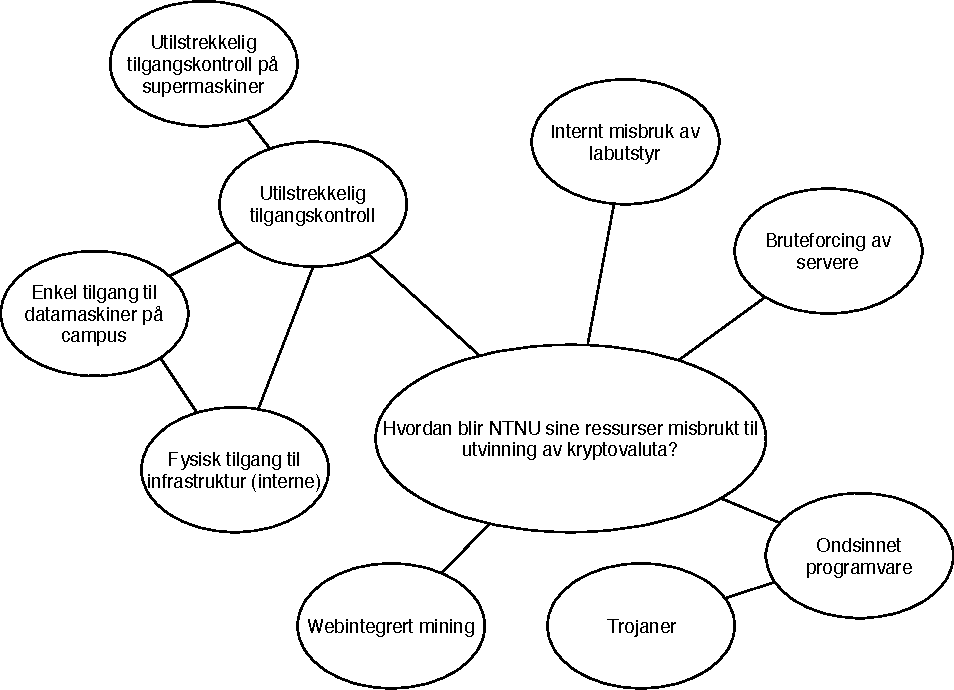
\includegraphics[scale=0.5]{case_3/bilder/idemyldring-hvordan.pdf}
    \caption[Idémyldring]{Resultater og gruppering av Hvordan}
     \label{fig:idemyldring-hvordan}
\end{figure}

\begin{figure}[H]
    \centering
    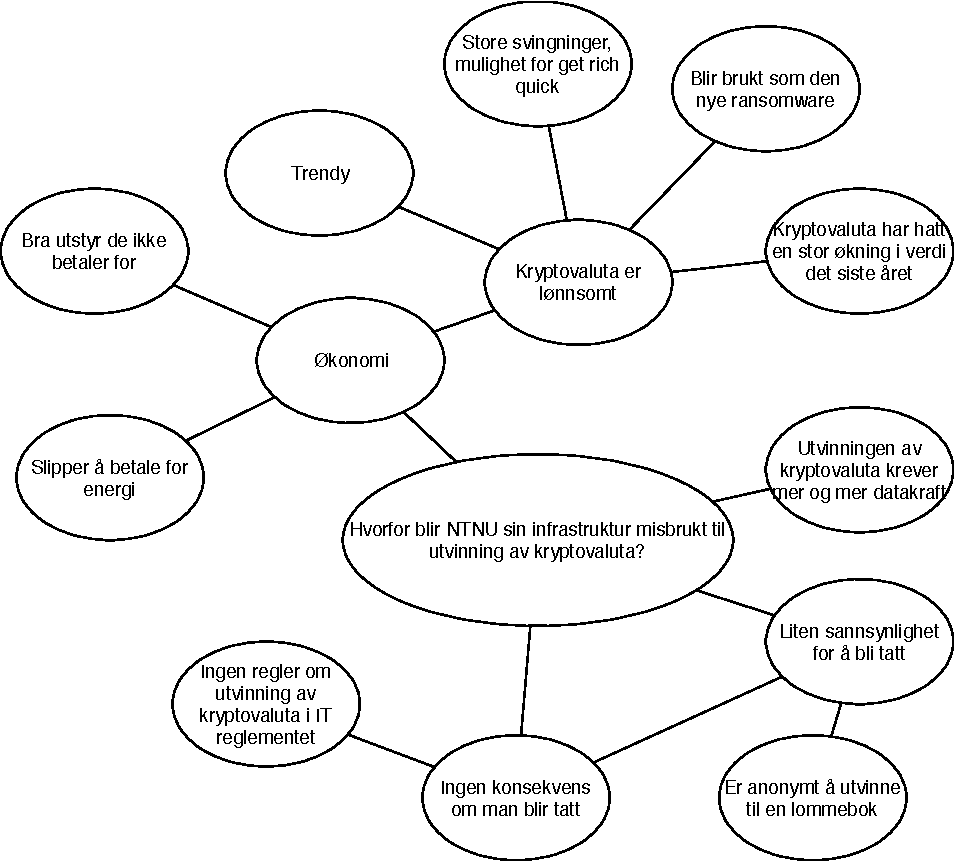
\includegraphics[scale=0.5]{case_3/bilder/idemyldring-hvorfor.pdf}
    \caption[Idémyldring]{Resultater og gruppering av Hvorfor}
    \label{fig:idemyldring-hvorfor}
\end{figure}

RESULTAT

\subsection{Konklusjon av verktøyet}
Verktøyet hjelper til med å få økt forståelse på hva som er årsaker til problemstilingen eller i denne samenheng to problemstilinger. Finnes det en klar problemstiling er det lett å komme med ideer på hva som er årsakene. Det gir et god overordnet bilde av situasjonen, men siden vi har lite tid på dette caset kommer det veldig mange idéer, der noen trolig blir unødvendige å følge.



\section{Nominell gruppeteknikk}
Nominell gruppeteknikk anbefales dersom det er idéer som må prioriteres. 

\subsection{Ønsket utbytte}
Siden vi hadde dårligere tid på dette caset enn på de tidligere, har vi valgt å benytte NGT for å prioritere idéer.

\subsection{Gjennomføring}
NGT ble utført med at vi alle satt oss ned sammen og hadde 15 poeng hver å gi til forskjellige idéer. Idéene ble laget utifra forarbeidet som var blitt gjort i idémyldringsprosessen, de idéene som lignet på hverandre ble slått sammen og noen ble litt omformulert. Idéene skulle få poengene 1, 2, 3, 4 eller 5 og alle disse 15 poengene skulle gis ut. Hver person ga ut sine 15 poeng for hva de trodde ville være det viktigste å fokusere på videre i analysen, og disse dataene kan sees i tabell \ref{tab:NGT}.

\subsection{Resultater}
Etter at hvert gruppemedlem hadde gitt ut sine 15 poeng satt vi igjen med 4 idéer som stakk seg ut med hvor mange poeng de fikk, disse er i fet skrift i tabell \ref{tab:NGT}. Disse fire årsakene er de vi kommer til å fokusere på i dette caset. De fire fokuspunktene kan deles etter de to problemstillingene ``hvordan og hvorfor''.

De to årsakene knyttet til ``hvorfor problemstillingen'' går ut på at det ikke er ulovlig med kryptoutvinning i henhold til gjeldende regelverk og faller derfor i en gråsone, der en ikke får noen represalier for å holde på med kryptoutvinning, annet enn å bli kastet av nettet.

De neste årsakene går ut på hvilke aktører som bruker universitetet sine ressurser til utvinning av kryptovaluta, og hvordan de bruker ressursene. Internt misbruk av labutstyr går ut på at studenter eller ansatte har tilgang til diverse labber og PCer som kan brukes til utvinning av kryptovaluta. Både ondsinnet programvare som utvinner kryptovaluta og webintegrerte utvinnere gjøres av eksterne aktører. Pengene som tjenes her går som regel tilbake til diverse kriminelle nettverk. Det med utvinning av kryptovaluta har blitt mye mer utbredt som et alternativ til ransomware. Ransomware har blitt mindre lønnsomt i den siste tiden \cite{RW}.

\begin{table} [H]
    \begin{tabular}{ | m{2em} | m{30em} | m{3em} | }
        \hline
            \cellcolor{yellow}  & \cellcolor{yellow} \textbf{Årsak} & \cellcolor{yellow} Poeng \\
        \hline
           A& Bra utstyr de ikke betaler for & 5 \\
        \hline
          B & Bruteforce av servere & 0 \\
        \hline
          C & Enkel tilgang til datamaskiner på campus & 0 \\
        \hline
         \textbf{D} & \textbf{Ingen regler om utvinning av kryptovaluta i IT reglementet} & 11 \\
        \hline
          \textbf{E} & \textbf{Internt misbruk av labutstyr} & 8  \\
        \hline
          F & Kryptovaluta har hatt en stor økning i verdi det siste året & 0 \\
        \hline
         G & Liten sannsynlighet for å bli tatt & 2 \\
        \hline
         \textbf{H} & \textbf{Ondsinnet programvare som miner} &  16 \\
        \hline
         I & Slipper å betale for energi & 0 \\
        \hline
         J & Store svingninger, mulighet for “get rich quick" & 0 \\
        \hline
         K & Utilstrekkelig tilgangskontroll på supermaskiner & 0 \\
        \hline
         L & Utvinningen av kryptovaluta krever mer og mer datakraft & 4 \\
        \hline
         \textbf{M} & \textbf{Webintegret miner} & 14 \\
        \hline
    \end{tabular}
    \caption{Oversikt over prioritering av idéer ved hjelp av NGT}
    \label{tab:NGT}
\end{table}

\subsection{Konklusjon av verktøyet}
Verktøyet hjelper til med å bestemme hvilke idéer fra tidligere idémyldring det er viktig å følge videre i prosessen. Det negativt med denne metoden, er at alle har like mye de skulle ha sagt om en sak, selvom de kanskje ikke har like mye kunnskap om de forskjellige momentene. Det positive er at vi får prioritert årsakene i henhold til viktighet. 
\chapter{Datainnsamling}
Målet i denne fasen er å samle inn et så bredt aspekt av informasjon som mulig gjennom et par mulige verktøy og teknikker beskrevet i boka om rotårsaksanalyse\cite{RCA}. Dette kapittelet går inn på hvordan informasjonen til caset ble samlet inn.
\chapter{Dataanalyse}
I denne fasen analyseres vi dataene som er samlet inn, vi har ganske lite data i dette caset, derfor har vi ganske få valgmuligheter for bruk av verktøy i følge boken \cite{RCA}. Dataene er heller ikke på nummerisk form, som flere av analyseverktøyene krever.

\section{Affinitetsdiagram}
Affinitetsdiagram brukes til å analysere data som det ikke er mulig å nummerere, eksempelvis meninger eller ideer. Affinitetsdiagram grupperer data og finner de underliggende korrelasjoner og likhetstrekk i gruppen.


\section{Ønsket utbytte}
Ønsket utbytte av å bruke affinitetsdiagram er å finne bindinger eller fellesnevnere som kan være til hjelp for å fjerne rotårsaken. 

\section{Gjennomføring}
Analysen ble gjennomført med å ta transkripsjon av intervjuet og stykke den opp i fem hovedgrupper.     

\section{Resultat}

\begin{figure}[H]
    \centering
    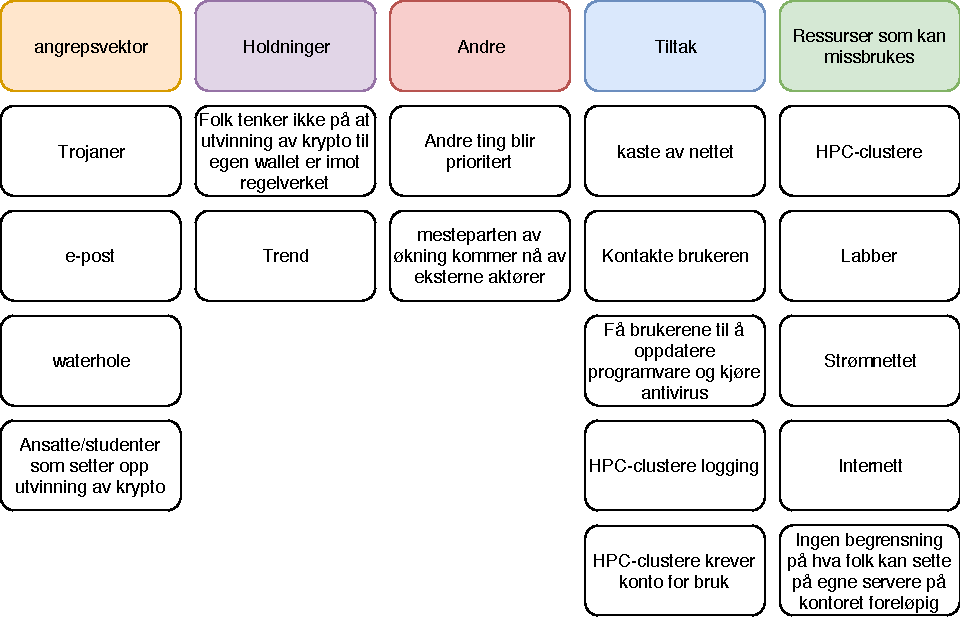
\includegraphics[scale=0.6]{case_3/bilder/AD.pdf}
    \label{fig:AD_miner}
    \caption[Analyse av intervju]{Hvordan fungerer utvinning av kryptovaluta ved NTNU?}
\end{figure}

Vi finner mulige årsaker og tiltak som er satt på plass, og forhåpentligvis er rotårsaken blant dem.

\section{Konklusjon av verktøy}
Verktøyet fungerte godt, selv med en liten datamengde. Vektøyet er effektivt til å strukturere transkripsjonen fra intervjuet til mer brukbare og oversiktlige nøkkelpunkter. 

\chapter{Rotårsaksidentifisering}
Arbeidet i denne fasen går ut på å identifisere rotårsaken. I foregående fasen ble en rekke mulige årsaker identifisert og analysert, men nå er det tid for å finne den faktiske rotårsaken. Det er mange forskjellige verktøy som kan brukes i denne fasen, men vi har brukt et 5 whys og feiltreanalyse for vårt utgangspunkt. 

\section{5 whys}
5 Whys er et verktøy som prøver å gjøre et dypdykk i årsakene for å finne rotårsaken. Måten dette gjøres på er å hele tiden spørre ``Why?'', altså hvorfor på norsk, hver gang en ny årsak dukker opp. Det brukes ofte for å sjekke om de identifiserte årsakene er symptomer, lav-nivå årsaker eller rotårsaker. 

\subsection{Ønsket utbytte}
Ved å bruke 5 Whys ønsker  vi å finne ut hva som er rotårsaken til problemet. Målet her er å få frem så mange rotårsaker som mulig, som vi kan bruke på rotårsakselimineringen. 

\subsection{Gjennomføring}
Med dette verktøyet tar vi utgangspunkt i casebeskrivelsen; nemlig rotårsaken til kryptoutvinning på NTNU. Ut fra dette brukte vi funnene fra analysen for å komme på årsaker, samt prøvde å idémyldre et par nye. For hver av disse årsakene ble det spurt: ``Hvorfor er dette en årsak av det originale problemet?''. For hvert svar spør vi hvorfor igjen og igjen helt til vi finner rotårsaken. Det ble tatt utgangspunkt i fem iterasjoner, men det er mulighet for flere eller færre avhengig av om spørsmålet kan besvares på en fornuftig måte. 

\subsection{Resultater}
Det ble fremhevet fem årsaker som skulle analyseres. Fire av disse kom fra fiskebeindiagrammet over, og en fra idémyldring. Tabellene under viser resultatene fra gjennomføringen. 

\begin{table} [H]
    \centering
    \begin{tabular}{ | m{5em} | m{30em} | }
        \hline
            \cellcolor{yellow} Årsak: & \cellcolor{yellow} Ansatte og studenter utvinner krypto med universitetet sine ressurser                \\
        \hline
            Why? & Lønnsomhet                                    \\
        \hline
            Why? & Har ingen utgifter                                            \\
        \hline
            Why? & Bruker strøm og infrastrukturen til skolen                \\
        \hline
            Why? & Det er en gråsone i regelverket           \\
        \hline
            Why? & Ikke spesifisert godt nok i IT-reglementet   \\
        \hline
    \end{tabular}
    \caption[5 Whys: Ansatte og studenter utvinner krypto med skolens]{5 Whys på ansatte og studenter utvinner krypto med skolens}
    \label{5Whys-interne}
\end{table}
Det å utvinne krypto på universitetet sine ressurser er alt fra å kjøre en kryptominer på en PC til å sette opp en mining rig. I 5 Whys over kom vi frem til at lønnsomhet er primærgrunnen til at de driver med kryptoutvinning, men årsaken til at ansatte og studenter utvinner på universitet er at det ikke er spesifisert godt nok i IT-reglementet.   


\begin{table} [H]
    \centering
    \begin{tabular}{ | m{5em} | m{30em} | }
        \hline
            \cellcolor{yellow} Årsak: & \cellcolor{yellow} Eksterne trusselaktører utvinner krypto med skolens ressurser              \\
        \hline
            Why? & Lønnsomhet                                   \\
        \hline
            Why? & Enkelt å spre minere                                           \\
        \hline
            Why? & Folk går inn på waterholes og trykker på phishingmail               \\
        \hline
            Why? & Brukeren var ikke oppmerksom nok på e-mailen eller siden de gikk på           \\
        \hline
            Why? & Brukere har ikke fått nok opplæring i hvordan dette unngås    \\
        \hline
    \end{tabular}
    \caption[5 Whys: Eksterne trusselaktører utvinner krypto med skolens ressurser]{5 Whys Eksterne trusselaktører utvinner krypto med skolens ressurser}
    \label{5Whys-eksterne}
\end{table}

Årsaken til at eksterne trusselaktører utvinner krypto med skolen sine ressurser er fordi det er en lønnsom affære som er koster lite å distribuere og som det er liten sannsynlighet for å bli tatt for. Med eksterne trusselaktører mener vi folk som utvinner på andre sine datamaskiner gjennom å få skadevare installert på disse.

\begin{table} [H]
    \centering
    \begin{tabular}{ | m{5em} | m{30em} | }
        \hline
            \cellcolor{yellow} Årsak: & \cellcolor{yellow} Utvinnere som implementert inn i nettsider              \\
        \hline
            Why? & God fortjeneste                                   \\
        \hline
            Why? & Fordi de når en stor menge folk som utvinner krypto for dem                                           \\
        \hline
            Why? & Mange har ikke en annonseblokkering som også stopper utvinnere på nett               \\
        \hline
            Why? & På grunn av lite eller ingen opplæring til denne typen programvare           \\
        \hline
            Why? & Ikke prioritert    \\
        \hline
            Why? & Fordi det ikke er nok folk/ressurser    \\
        \hline
    \end{tabular}
    \caption[5 Whys: Minere som er implementert inn i nettsider]{5 Whys på ansatte og studenter utvinner krypto med skolens}
    \label{5Whys-minere}
\end{table}
Utvinning på nettsider blir mer utbredt fordi det er profitabelt og en god erstatning til reklame. Dette kan bli stoppet med annonseblokkering eller blokkering av DNS adresser. Dette blir ikke gjort fordi det ikke er en prioritet fra seksjon for digital sikkerhet.

%Årsaken til at nettsider som har muligheten til å utvinne kryptovaluta er et problem fordi, de starter å bli utbredt og de spør ofte ikke om godkjenning for utvinning på PCer.

\subsection{Konklusjon av verktøy}
Verktøyet var svært nyttig for å gå dypt inn i årsakene. Et problem består ofte av flere nivåer av årsaker, og det tar 5 Whys hensyn til. I forhold til informasjonssikkerhet burde man passe på å ikke alltid ende opp med en årsak som er relatert til IT-reglement, da problemet ofte også kan være av teknisk art. Et problem med verktøyet er at det kan bli for ensporet på en spesifikk tankegang. Det kan derfor anbefales i noen tilfeller å undersøke samme årsaken flere ganger dersom det er grunn til å tro at det finnes flere relevante årsaker ved ett av spørsmålene, som fører til en annen rotårsak.

\section{Feiltreanalyse}
Feiltreanalyse tar alle mulige årsaker i et diagram og identifiserer mulige linker. Analysen bygger på hva som ble gjort i 5 Whys. 

\subsection{Ønsket utbytte}
Ved bruk av dette verktøyet ønsker vi å få en oversikt over koblinger mellom de forskjellige årsakene. Vi ønsker også å få sortert ut de årsakene som NTNU ikke har mulighet til å gjøre.

\subsection{Gjennomføring}
Med dette verktøy tar vi utgangspunktet i resultatet fra 5 Whys til å finne rotårsakene. Her går vi steg for steg nedover og ser på hva som er årsaken til at enhver uønsket hendelse inntreffer.

\subsection{Resultater}
Vi har kommet fram til fire hovedgrunner til at kryptoutvinning på NTNU forekommer. Rotårsaken er sammensatt av disse årsakene definert i figur \ref{fig:feil_tre_analyse}. I dette caset er problemet delt inn i to deler; de interne og de eksterne. Det er to forskjellige typer årsaker, der interne går mer på regelverk og eksterne er mer teknisk.          

I figur \ref{fig:feil_tre_analyse} representerer trekanter ``eller'', halvsirkelen representer ``og''. De røde boksene er de årsakene vi ikke kan gjøre noe med, de grønne kan det gjøres noe med.
 \begin{figure}[H]
    \centering
    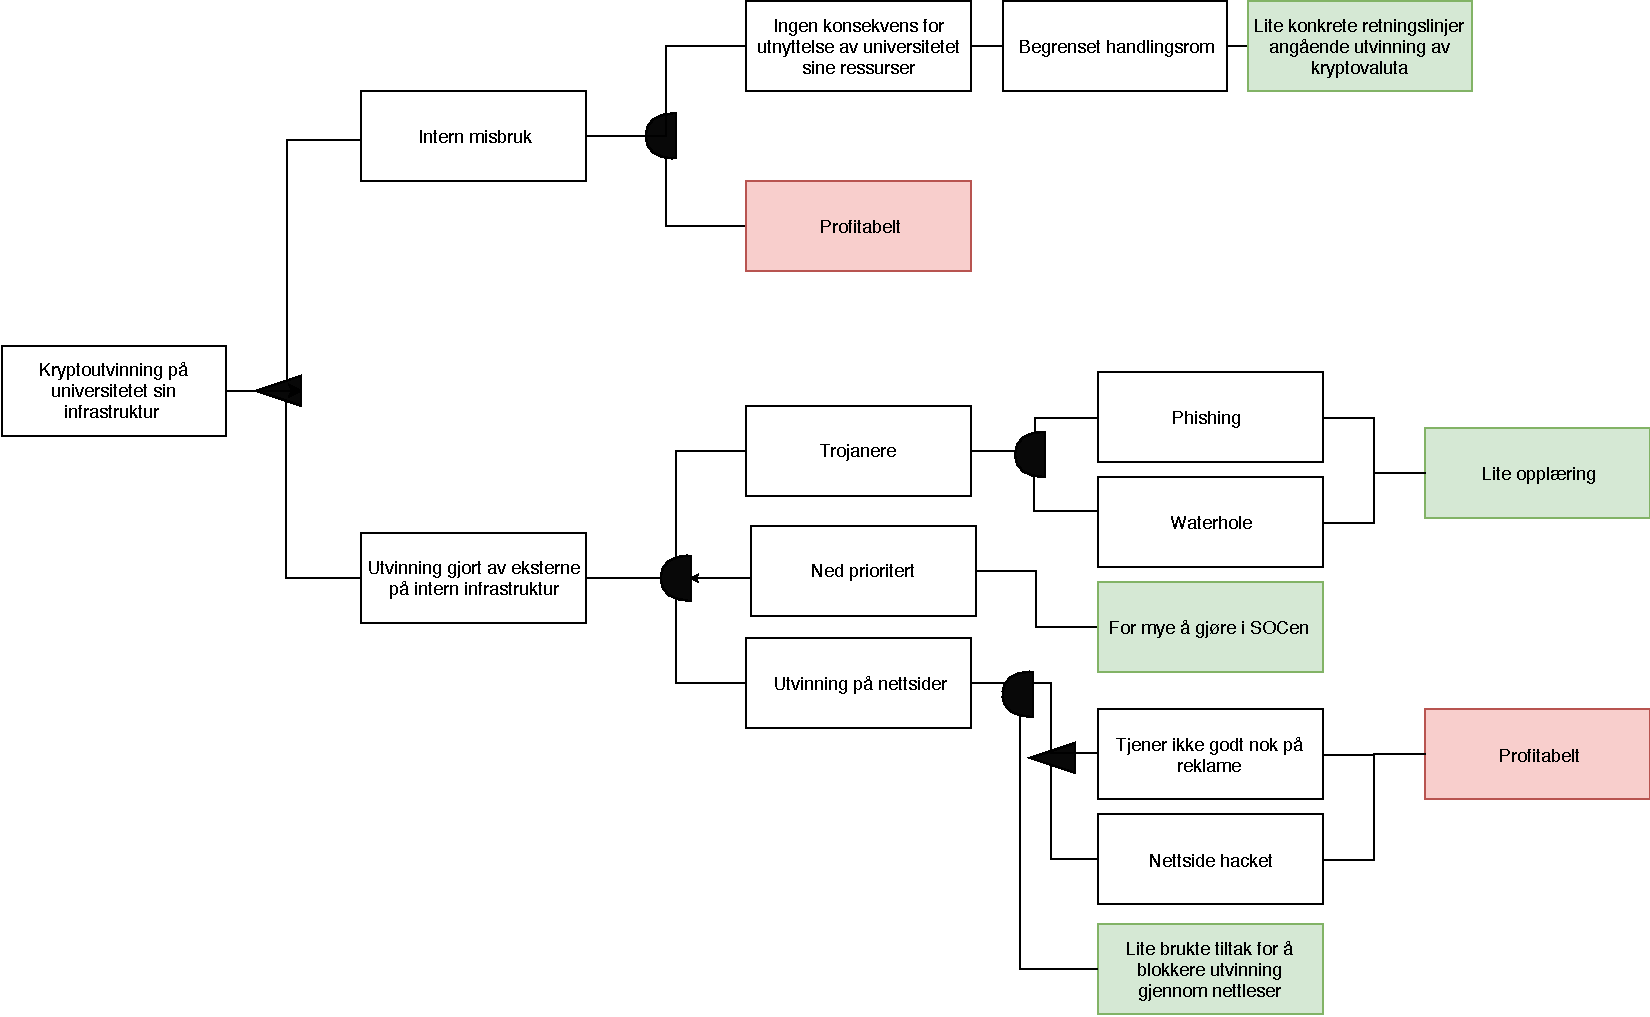
\includegraphics[scale=0.45]{case_3/bilder/feil_tre_analyse.pdf}
    \caption[Feiltreanalyse]{Feiltreanalyse}
    \label{fig:feil_tre_analyse}
\end{figure}

\subsection{Konklusjon av verktøy}
Verktøyet funger godt til å se hvordan de forskjellige årsakene er koblet sammen og hva som er hovedårsakene.
\chapter{Rotårsakseliminering}
\chapter{Løsningsimplementering}
Arbeidet i denne fasen går ut på å utrede en tiltaksplan og lage et forslag til hvordan dette skal implementeres. I den foregående fasen ble løsningene til rotårsakene identifisert. Vi kom fram til fire tiltak som vil fjerne rotårsaken. Tiltakene kan deles inn i to deler, en for eksterne og en for interne. Den eksterne løsningen går på det tekniske og den interne går på IT-reglementet. 

Den eksterne løsningen er å øke ressursene til seksjonen for digital sikkerhet gjennom å ansatte flere eller å bruke bachelorstudenter til å utføre blokkering av DNS-forespørsler tilknyttet kryptoutvinning.

Den interne løsningen er å tydeliggjøre at det å drive kryptoutvinning på NTNU ikke er lovlig og gjennomføre enn informasjonskampanje rundt dette.

\section{Kraftfeltsanalyse}
Kraftfeltsanalyse er et verktøy som analyserer hva som hjelper og hva som hindrer implementering av tiltaket.  

\subsection{Ønsket utbytte}
Ønsket utbytte fra kraftfeltsanalyse er å få vite hva som er for og hva som er imot implementering av tiltakene. Dette verktøyet gir en plan over hvilke tiltak som er lettest å gjennomføre. 

\subsection{Gjennomføring}
Kraftfeltsanalysen ble gjort ved at vi tok tiltakene fra problemelimineringen og hadde en idémyldring for å se hva som talte for tiltakene og hva som var imot. 

\subsection{Resultat}
 Under har vi de fire kraftfeltsanalysene
 
 Informasjonskampanjen og endringen i IT-reglementet bør gjøre i kombinasjon med hverandre. Der IT-reglementet får klartgjort at selv om kryptoutvinning ikke ulovlig i henhold til norsk lov, er det imot NTNU sitt IT-reglement så langt det ikke er søkt om. Når endringen er gjort, gjennomføres informasjonskampanjen.   
 Under, i tabell \ref{fig:kampanje} og \ref{fig:IT-reglement}, viser resultatene fra kraftfeltsanalyse på informasjonskampanje og endring i IT-reglementet.
 \begin{figure}[H]
    \hspace{2.2cm}
    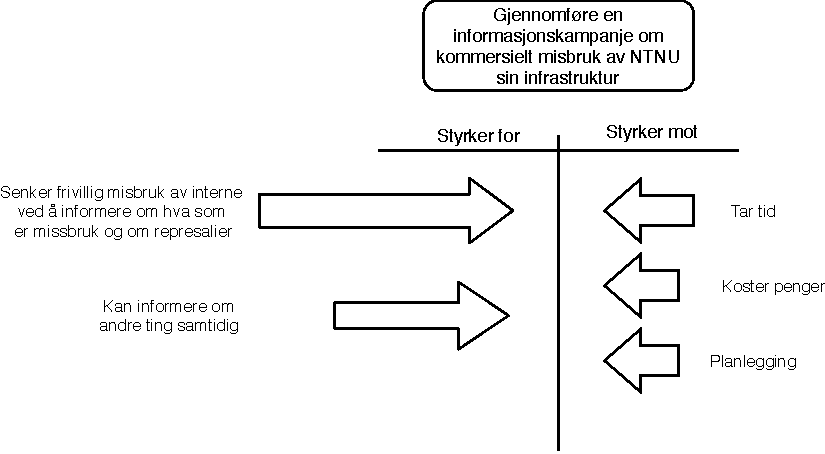
\includegraphics[scale=0.6]{case_3/bilder/Force-field1.pdf}
    \caption[Informasjonskampanje]{Oversikt over informasjonskampanjen }
    \label{fig:kampanje}
\end{figure}

 
 \begin{figure}[H]
    \hspace{2.6cm}
    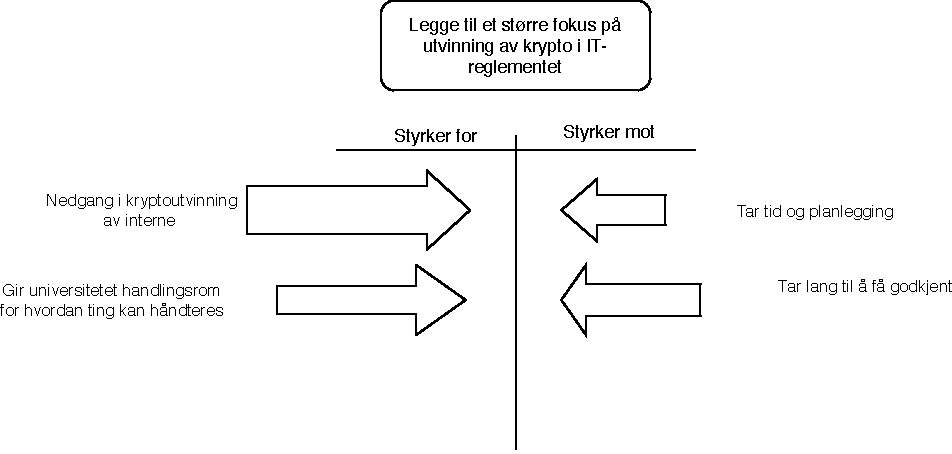
\includegraphics[scale=0.6]{case_3/bilder/Force-field2.pdf}
    \caption[Endre IT-reglementet]{Endring i IT-reglementet}
    \label{fig:IT-reglement}
\end{figure}

Fra dataanalysen kom fram til at selv om det finnes tekniske løsninger, har ikke SOCen hatt mulighet til å implementere DNS blokkering på bakgrunn av mangel på ressurser. Figur \ref{fig:Blokkering} og \ref{fig:Oke-antall} viser hva som skal til for å blokkere DNS og hva som må til for å øke ressursene til SOCen.    
 \begin{figure}[H]
    \centering
    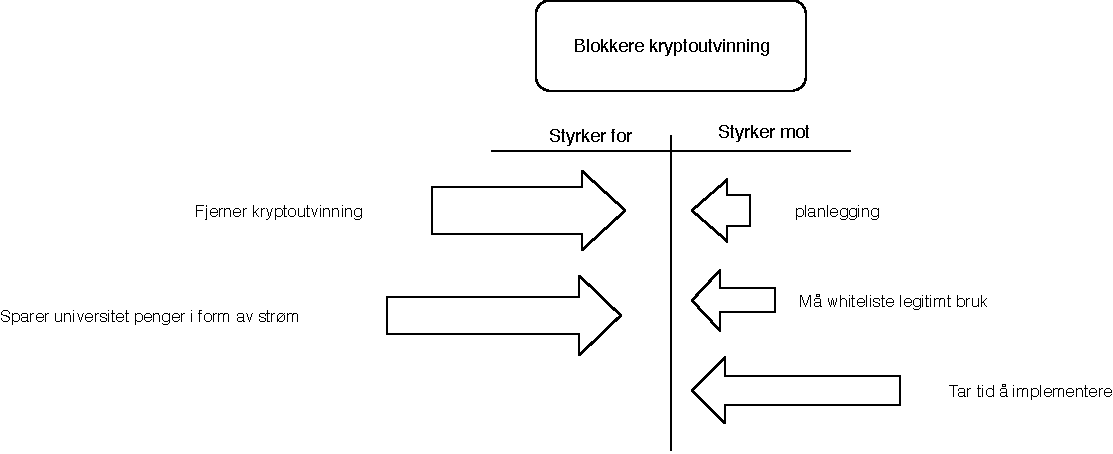
\includegraphics[scale=0.6]{case_3/bilder/Force-Field3.pdf}
    \caption[Blokkering]{Blokkering av DNS forespørsel}
    \label{fig:Blokkering}
\end{figure}

 \begin{figure}[H]
    \hspace{3.6cm}
    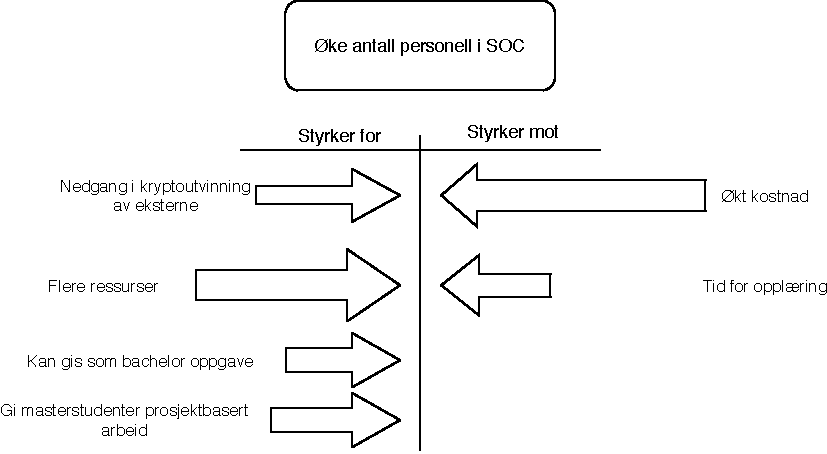
\includegraphics[scale=0.6]{case_3/bilder/Force-field4.pdf}
    \caption[Øke antall ansette i SOC]{Øke andel ansatte i SOC}
    \label{fig:Oke-antall}
\end{figure}

Figurene viser våres antakelser på hva som jobber for implementeringen og hva som jobber imot samt  estimater på styrken til antakelsene. 
\subsection{Konklusjon av verktøyet}
Verktøyet har potensiale til å fungere bra, der oversikten man får er bra så lenge datagrunnlaget er godt. Problemmet vårt var at vi jobbet med antakelser og ikke et datasett. Vi hadde ikke tid til å undersøke estimatene, så de har en høy usikkerhet.     
\chapter{Diskusjon og konklusjon}

\chapter{Vedlegg: Transcript av intervju}
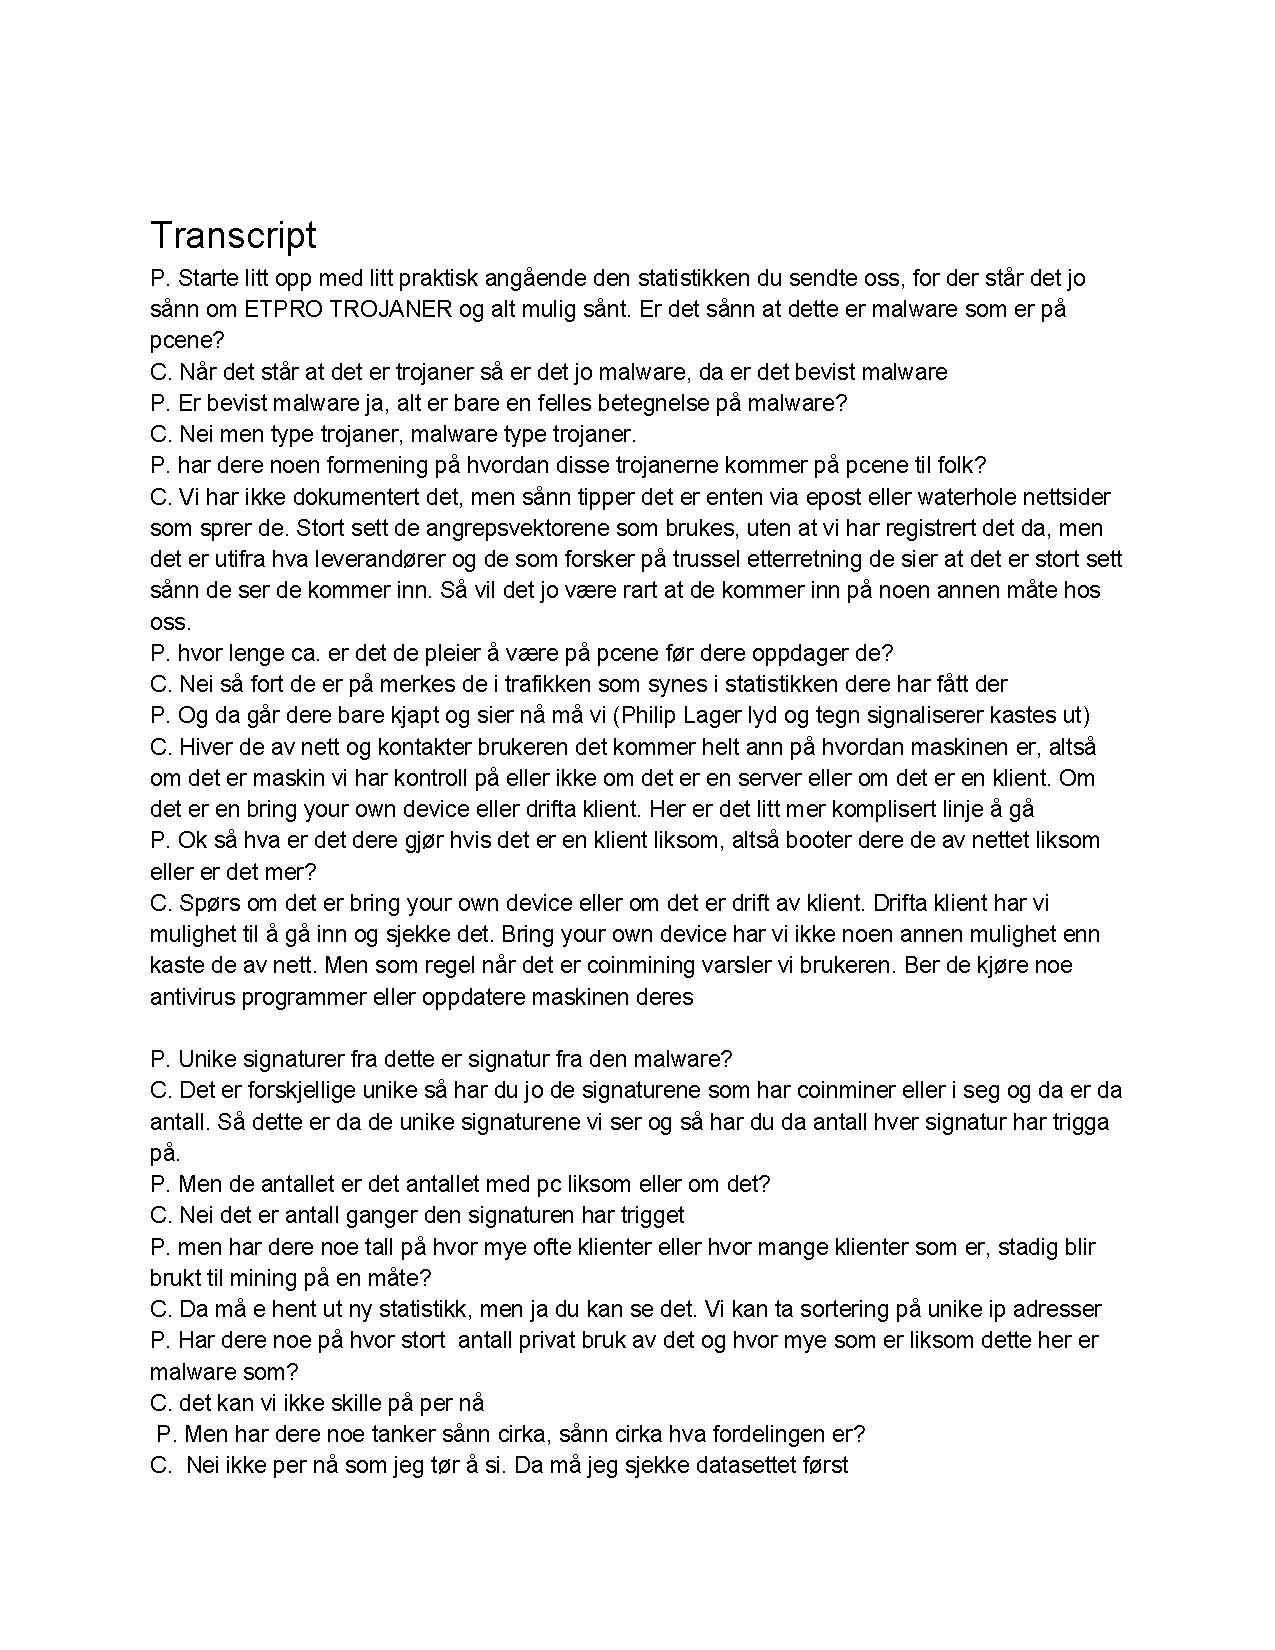
\includepdf[pages=1-3]{bilder/transcript.pdf}
\label{Transcript_intervju}

\bibliographystyle{ntnuthesis/ntnubachelorthesis}
\bibliography{case_3/bibliografi}

\appendix %after this line all chapters will have leters instead of numbers
%\input{projectplan}
%\input{gantt}
%\chapter{Meeting Logs}
You should include in the Appendix a log of your meeting.
\section{Temporal record of meetings}
\subsection*{11.01.2016 - Bachelor Information Meeting}
Discussion of the process and setup of the thesis.  Deadlines for submission of documentation.  Introduction to the process and the sessions to help with writing the thesis....

\subsection*{12.01.2016}
Met with supervisor to discuss the project. Actions:
\begin{enumerate}
	\item decide on a writing tool
	\item install development environment
	\item draft agreements by next week.
\end{enumerate}



%\input{progressreviews}
%\input{worklog}

\end{document}